\documentclass[11pt]{article}
\title{\textbf{Meccano hexagons}}
\author{https://github.com/heptagons/meccano/hexa}
\date{}

\usepackage{amsmath}
\usepackage{listings}
\usepackage{xcolor}
\definecolor{gray}{RGB}{245,245,245}

\lstset{
	backgroundcolor=\color{gray},
	frame=single,
	numbers=left,
	stepnumber=1,
	tabsize=2,
	basicstyle=\ttfamily\small,
	breaklines=true
}

\usepackage[margin={0.75in}]{geometry}

\usepackage{tikz}
\usetikzlibrary{math}

\usepackage{graphicx}
\usepackage{hyperref}
\usepackage{multicol}

\begin{document}

\maketitle
\begin{abstract}
We construct meccano\footnote{
\href{https://webspace.science.uu.nl/~hooft101/lectures/meccano.pdf}{Meccano mathematics by `t Hooft }
}
regular hexagons.
We use six equal strips to build the polygon perimeter and then we attach \textbf{internal diagonals} to make the polygon regular and rigid. Common diagonals called \textbf{
regular diagonals} are aligned with the common equilateral triangular grid and \textbf{
irregular diagonals} are not and are more interesting. To find the irregular diagonals
we develop algebraic formulas and run a program to do the search. Basically the problem
is to find triangles with the three integer sides and one angle exactly of $120^\circ{}$.
\end{abstract}

\section{Meccano hexagons}

\subsection {Regular diagonals}
A meccano hexagon can be build easily attaching sufficient equilateral
triangles as small as one unit side. 
Also joining six strips to form a perimeter and using two more strips as \textbf{regular diagonals},
which means both diagonals are aligned along the triangular grid.
Regular diagonals join opposite hexagon sides.

\begin{figure}[htpb]
\centering
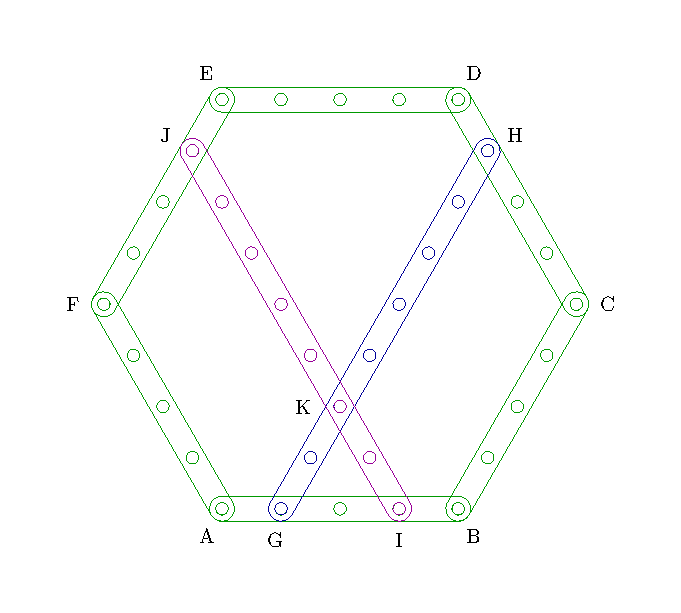
\includegraphics[scale=0.75]{hexagon_simple}
\caption{Hexagon of size $4$ with two \textbf{regular diagonals} of size $7$.}
\label{fig:regular}
\end{figure}

Consider figure \ref{fig:regular}.
Start with strip $\overline{AB}$ and add two strips $\overline{GH}$ and
$\overline{IJ}$ to form a triangle with three bolts at points $G$, $I$ and $K$. At this moment, perimeter points $A$, $B$, $H$ and $G$ are rigid.

Then add perimeter strips $\overline{BC}$ and $\overline{CD}$ with a bolt at $H$.
In the same way add perimeter strips $\overline{AF}$ and $\overline{EF}$ with a bolt at $J$.
Finally add strip $\overline{DE}$ with bolts at $D$ and $E$.



\begin{figure}[htpb]
\centering
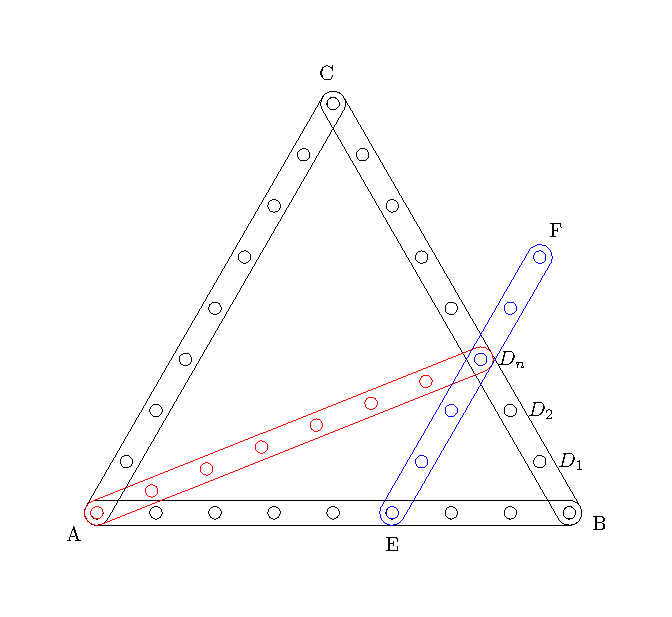
\includegraphics[scale=0.8]{hexagon_angle}
\caption{The red strip is an irregular diagonal, with integer length 
and joining two adjacent hexagon sides $\overline{AE}$ and $\overline{EF}$.}
\label{fig:irregular}
\end{figure}

\subsection{Irregular diagonals}

While regular diagonals are aligned along the triangular grid, \textbf{irregular diagonals}
don't. Irregular diagonals join two adjacent hexagon sides, making (rigid) irregular triangles.

Consider figure \ref{fig:irregular}.
Start with an equilateral triangle $ABC$ of side $\overline{AB}$.
Test one by one the irregular diagonals from the point $A$ to the points $D_1$, $D_2$..., $D_n$
which are over the strip $\overline{BC}$. Define the tree variables to use:
\begin{align*}
a &= \overline{AB}\\
b &= \overline{BD_n}\\
d &= \overline{AD_n}\\
\end{align*}
Acording to the cosines law and knowing the $\angle{EBD_n} = 60^\circ{}$, calculate $d$:
\begin{align*}
d &= \sqrt{a^2 + b^2 - 2ab\cos{\frac{\pi}{3}}}\\
  &= \sqrt{a^2 + b^2 - ab}\\
  &= \sqrt{(a-b)^2 + ab}\\
\end{align*}

Reject any non-integer diagonal $d$, since any meccano strip length should be an integer.
For the valid diagonal such as $\overline{AD_n}$, locate a point $E$ over the strip $\overline{AB}$
such so the distance $\overline{BE}$ equals the distance $\overline{BD_n}$.
From the point $E$ create a new strip $\overline{EF}$ passing over the point $D_n$ (blue strip in the figure).
Finally we got a valid \textbf{irregular diagonal} $d$ for the pair of adjacent
hexagon sides $\overline{AE}$ and $\overline{EF}$.

\subsection{Irregular diagonals program}

We need a program to iterate over integer $a$, then over integer $b$ to test whether $d$ value is an integer too.
Next golang program find the diagonals.
We iterate from $a=1$ to a given maximum (line 2).
Then we iterate over $1 < b \leq a/2$ (line 3), to avoid repeating symmetric values.
In order to reject repetitions by scaling we check for greatest commond divisor
of $a$ and $b$ to be $1$ (line 4).
Then we calculate the diagonal using the formula $d^2 = (a-b)^2 + ab$ (line 5) and report
only the case when the diagonal is a square number (line 8). 
\begin{lstlisting}
func triangle_diagonals(max int) {
  for a := 1; a < max; a++ {
    for b := 1; b <= a/2; b++ {
      if gcd(a, b) == 1 {
        diag := (a-b)*(a-b) + a*b
        cd := math.Sqrt(float64(diag))
        d := int(cd)
        if cd == float64(d) {
          num := float64(diag + a*a - b*b)
          den := 2.0 * cd * float64(a)
          angle := 180*math.Acos(num/den)/math.Pi
          fmt.Printf("a=%3d b=%3d d=%3d angle=%8.4f\n", a, b, d, angle)
        }
      }
    }
  }
}
func gcd(a, b int) int { // greatest common divisor
  if b == 0 {
    return a
  }
  return gcd(b, a % b)
}
\end{lstlisting}

\subsection{Irregular diagonals results}
The program found $13$ distinct irregular diagonals for sides $a \leq 100$.
Next table show the results including the angle $EAD_n$ needed for the latex drawing scripts.
\begin{lstlisting}
a=  8 b=  3 d=  7 angle= 21.7868
a= 15 b=  7 d= 13 angle= 27.7958
a= 21 b=  5 d= 19 angle= 13.1736
a= 35 b= 11 d= 31 angle= 17.8966
a= 40 b=  7 d= 37 angle=  9.4300
a= 48 b= 13 d= 43 angle= 15.1782
a= 55 b= 16 d= 49 angle= 16.4264
a= 65 b=  9 d= 61 angle=  7.3410
a= 77 b= 32 d= 67 angle= 24.4327
a= 80 b= 17 d= 73 angle= 11.6351
a= 91 b= 40 d= 79 angle= 26.0078
a= 96 b= 11 d= 91 angle=  6.0090
a= 99 b= 19 d= 91 angle= 10.4174
\end{lstlisting}

\newcommand{\strip}[4][000000]{ %[color]{n}{factor}{size}
 \definecolor{main}{HTML}{#1}
 \draw[main] (0,{{2*#4}})
   -- ++({#2*#3},0) arc(+90:-90:{2*#4})
   -- ++({-#2*#3},0) arc(270:90:{2*#4});
 \foreach \x in {0,1,...,#2}
  \draw[main] (\x*#3,0) circle (#4);
}

\newcommand{\resultA}[5]{ %{n}{diag}{factor}{size}{offset}
 \begin{tikzpicture}
  \def\r{21.7868}
  \begin{scope} %AB
   \strip[0000FF]{#1}{#3}{#4}
   \path (0,0) ++(240:5*#4) node{A};
   \begin{scope}[shift={(#5*#3,0)},rotate=\r] %AG
    \strip[FF6600]{#2}{#3}{#4}
    \path (#2*#3,0) ++(-45:5*#4) node{G};
   \end{scope}
   \begin{scope}[shift={(#1*#3,0)},rotate=60] %BC
    \strip[0000FF]{#1}{#3}{#4}
    \path (0,0) ++(240:5*#4) node{B};
   \begin{scope}[shift={(#5*#3,0)},rotate=\r] %BH
    \strip[FF6600]{#2}{#3}{#4}
    \path (#2*#3,0) ++(-60:5*#4) node{H};
   \end{scope}
  \begin{scope}[shift={(#1*#3,0)},rotate=60] %CD
   \strip[0000FF]{#1}{#3}{#4}
   \path (0,0) ++(240:5*#4) node{C};
   \begin{scope}[shift={(#5*#3,0)},rotate=\r] %CI
    \strip[FF6600]{#2}{#3}{#4}
    \path (#2*#3,0) ++(-60:5*#4) node{I};
   \end{scope}
   \begin{scope}[shift={(#1*#3,0)},rotate=60] %DE
    \strip[0000FF]{#1}{#3}{#4}
    \path (0,0) ++(240:5*#4) node{D};
     \begin{scope}[shift={(#1*#3,0)},rotate=60]
      \strip[0000FF]{#1}{#3}{#4}
      \path (0,0) ++(240:5*#4) node{E};
      \begin{scope}[shift={(#1*#3,0)},rotate=60] %EF
       \strip[0000FF]{#1}{#3}{#4}
       \path (0,0) ++(240:5*#4) node{F};
      \end{scope}
     \end{scope}
    \end{scope}   
   \end{scope}
  \end{scope}
 \end{scope}
\end{tikzpicture}
}

\newcommand{\resultB}[5]{ %{n}{diag}{factor}{size}{offset}
 \begin{tikzpicture}
  \def\r{27.7958}
  \begin{scope} %AB
   \strip[0088FF]{#1}{#3}{#4}
   \path (0,0) ++(240:5*#4) node{A};
   \begin{scope}[shift={(#5*#3,0)},rotate=\r] %AG
    \strip[990099]{#2}{#3}{#4}
    \path (#2*#3,0) ++(-45:5*#4) node{G};
   \end{scope}
   \begin{scope}[shift={(#1*#3,0)},rotate=60] %BC
    \strip[0088FF]{#1}{#3}{#4}
    \path (0,0) ++(240:5*#4) node{B};
   \begin{scope}[shift={(#5*#3,0)},rotate=\r] %BH
    \strip[990099]{#2}{#3}{#4}
    \path (#2*#3,0) ++(-60:5*#4) node{H};
   \end{scope}
  \begin{scope}[shift={(#1*#3,0)},rotate=60] %CD
   \strip[0088FF]{#1}{#3}{#4}
   \path (0,0) ++(240:5*#4) node{C};
   \begin{scope}[shift={(#5*#3,0)},rotate=\r] %CI
    \strip[990099]{#2}{#3}{#4}
    \path (#2*#3,0) ++(-60:5*#4) node{I};
   \end{scope}
   \begin{scope}[shift={(#1*#3,0)},rotate=60] %DE
    \strip[0088FF]{#1}{#3}{#4}
    \path (0,0) ++(240:5*#4) node{D};
     \begin{scope}[shift={(#1*#3,0)},rotate=60]
      \strip[0088FF]{#1}{#3}{#4}
      \path (0,0) ++(240:5*#4) node{E};
      \begin{scope}[shift={(#1*#3,0)},rotate=60] %EF
       \strip[0088FF]{#1}{#3}{#4}
       \path (0,0) ++(240:5*#4) node{F};
      \end{scope}
     \end{scope}
    \end{scope}   
   \end{scope}
  \end{scope}
 \end{scope}
\end{tikzpicture}
}

\begin{figure}
\centering
\scalebox{0.8}{
 \resultA{5}{7}{1}{3pt}{0}
}
\caption{Result 1. Hexagon side lenght: $5$, diagonal length: $7$.
This is the smallest hexagon of the results. The number of bolts is at minimum, 9.}
\label{fig:5-7}
\end{figure}

\begin{figure}
\centering
\scalebox{1}{
 \resultA{6}{7}{0.75}{3pt}{1}
}
\caption{Result 1. Hexagon side length: $5+1=6$, diagonal length: $7$. Has the same
diagonals of figure \ref{fig:5-7} but the perimeter was increased by one.
We need here 12 bolts.}
\label{fig:6-7}
\end{figure}

\begin{figure}
\centering
\scalebox{0.7}{
 \resultA{7}{7}{1.33}{3pt}{2}
}
\caption{Result 1: Hexagon sides $5+2=7$, diagonals $7$.
This is an interesting puzzle. Given nine strips of length 7, 
build a rigid regular hexagon. Notice how separated the holes should be in the strips
to prevent bolts conflicts near points $G$ and $H$. }
\label{fig:7-7}
\end{figure}

\begin{figure}
\centering
\scalebox{1}{
 \resultA{8}{7}{0.4}{3pt}{3}
}
\caption{Result 1: Hexagon sides $5+3=8$, diagonals $7$. This case is interesting
because adding three more orange strips we can make two rigid hexagons only when
both share bolts.}
\label{fig:8-7}
\end{figure}

\subsection{Examples of result 1}
Result 1 reports $a=8$, $b=3$ and $d=7$, so the diagonal is of length $7$ and the minimum hexagon size is $a - b = 5$.
Figure \ref{fig:5-7} shows the smallest hexagon with irregular diagonals.
In figure \ref{fig:6-7}, the side is incremented to $6$ and in figure \ref{fig:7-7}
the side is incremented to $7$ so all hexagon's strips are of the same length.
Finally in figure \ref{fig:8-7}, the size is incremented to $8$ and we see two
hexagons at the same time of sizes $7$ and $8$.


\begin{figure}
\centering
\scalebox{1}{
 \resultB{8}{13}{0.5}{3pt}{0}
}
\caption{Result 2. Hexagon sides: $8$, diagonals: $13$.}
\label{fig:8-13}
\end{figure}

\begin{figure}
\centering
\scalebox{1}{
 \resultB{15}{13}{0.4}{3pt}{7}
}
\caption{Hexagon sides $8+7=15$, diagonals $13$.}
\label{fig:15-13}
\end{figure}

\subsection{Examples of result 2}
Result 2 reports $a=15$, $b=7$ and $d=13$, so the diagonal is of length $13$ and the minimum
hexagon size is $a - b = 8$. Figure \ref{fig:8-13} shows the smallest hexagon with irregular
diagonal $13$ and figure \ref{fig:15-13} extends the side from $8$ to $15$ and we see two
hexagons at the same time of sizes $13$ and $15$.

\subsection{Results longer list}
This list shows $s = a-b$ which is the side of each hexagon, $b$ the segment of the
second side and the diagonal $d$ which is the triangle side opposite to the angle of $120^\circ{}$. $ d > s > b$.
\setlength{\columnsep}{100pt}
\begin{multicols}{2}
\begin{lstlisting}
s=  5 b=  3 d=  7
s=  8 b=  7 d= 13
s= 16 b=  5 d= 19
s= 24 b= 11 d= 31
s= 33 b=  7 d= 37
s= 35 b= 13 d= 43
s= 39 b= 16 d= 49
s= 56 b=  9 d= 61
s= 45 b= 32 d= 67
s= 63 b= 17 d= 73
s= 51 b= 40 d= 79
s= 85 b= 11 d= 91
s= 80 b= 19 d= 91
s= 57 b= 55 d= 97
s= 77 b= 40 d=103
s= 95 b= 24 d=109
s=120 b= 13 d=127
s=120 b= 23 d=133
s= 88 b= 65 d=133
s= 91 b= 69 d=139
s=143 b= 25 d=157
s=115 b= 56 d=151
s=161 b= 15 d=169
s=112 b= 75 d=163
s=175 b= 32 d=193
s=105 b=104 d=181
s=165 b= 56 d=199
s=195 b= 29 d=211
s=208 b= 17 d=217
s=160 b= 87 d=217
s=168 b= 85 d=223
s=224 b= 31 d=241
s=145 b=119 d=229
s=203 b= 72 d=247
s=261 b= 19 d=271
s=187 b= 93 d=247
s=221 b= 64 d=259
s=155 b=144 d=259
s=217 b= 95 d=277
s=279 b= 40 d=301
s=288 b= 35 d=307
s=192 b=133 d=283
s=320 b= 21 d=331
s=209 b=136 d=301
s=247 b=105 d=313
s=323 b= 37 d=343
s=272 b=105 d=337
s=280 b=111 d=349
s=315 b= 88 d=367
s=385 b= 23 d=397
s=231 b=185 d=361
s=273 b=152 d=373
s=259 b=176 d=379
s=357 b= 80 d=403
s=399 b= 41 d=421
s=333 b=115 d=403
s=407 b= 48 d=433
s=304 b=161 d=409
s=352 b=123 d=427
s=456 b= 25 d=469
s=440 b= 43 d=463
s=253 b=240 d=427
s=299 b=205 d=439
s=391 b=129 d=469
s=437 b= 88 d=487
s=287 b=240 d=457
s=369 b=175 d=481
s=336 b=215 d=481
s=451 b=104 d=511
s=533 b= 27 d=547
s=528 b= 47 d=553
s=301 b=275 d=499
s=325 b=264 d=511
s=387 b=208 d=523
s=473 b=135 d=553
s=425 b=184 d=541
s=559 b= 56 d=589
s=475 b=141 d=559
s=575 b= 49 d=601
s=440 b=189 d=559
s=616 b= 29 d=631
s=416 b=235 d=571
s=368 b=297 d=577
s=520 b=147 d=607
s=351 b=329 d=589
s=552 b=145 d=637
\end{lstlisting}

\end{multicols}

\end{document}
